\documentclass{beamer}
%\usetheme{Antibes}
%\usetheme{Dresden}
\usetheme{Frankfurt}
%\usetheme{Copenhagen}
%\usetheme{Darmstadt}
%\usecolortheme{dolphin}
\usepackage{cancel}
\usepackage{tikz}
%%%%%%%%%%%%%%%%%%%%%%%%%%%%%%%%%%%%%%%%%%%%%%%%%%%%%%%%
\usepackage{multicol}

\newtheorem{proposition}[theorem]{Proposition}
\newtheorem{remark}[theorem]{Remark}
\newtheorem*{remark*}{Remark}
\newtheorem{conjecture}[theorem]{Conjecture}
\newtheorem{claim}[theorem]{Claim}
\newtheorem*{claim*}{Claim}
\usepackage{xcolor}
\usepackage{longtable}
\usepackage{hyperref}
\newtheorem{openproblem}[theorem]{Open Problem}


\setbeamertemplate{blocks}[rounded][shadow=true]

\setbeamertemplate{theorems}[ams style]
\begin{document}
	\title[]{\textcolor{black}{\textbf{Linear Regression Analysis for the Kings County's (Seattle, WA) House Market.}}}
	
	\author[Yevgeniy Kostrov \hspace{1in} kostrovy@mville.edu]
	{\textcolor{black}
	{\textbf{by Y.~Kostrov\inst}}}
	\date[April 14, 2019]

%
%	Title Page:
%	

%	{
%\usebackgroundtemplate{\includegraphics[height=\paperheight,width=\paperwidth]{london}}
%\frame{
%}
%}
	\begin{frame}	
			\maketitle
	\end{frame}
\begin{frame}{\contentsname}
	\begin{multicols}{2}
		\tableofcontents
	\end{multicols}
\end{frame}
%
%
%	
%
%
%}
\section{Overview}
\frame{
\frametitle{Overview }
\begin{center}
	The purpose of this project is to analyze a data set containing data about houses sold in Kings County (Seattle, WA).
\end{center}
}
\frame{
	\frametitle{Overview }
During the analysis:
\pause
\begin{enumerate}
	\item I will perform necessary data wrangling first.
	\pause
	\item I will build a Linear Regression Model with one explanatory variable.:
	\pause
		\begin{itemize}
			\item I will check statistical assumptions for the linear regression model
			\item I will explain the model, including intercept, coefficient for the explanatory variable, $R^2$, and ANOVA
		\end{itemize}
	\pause
	\item I will build a Multiple Linear Regression Model with many explanatory variables.
	\pause
	\begin{itemize}
		\item I will check statistical assumptions for the multiple linear regression model
		\item I will explain the model, including intercept, coefficients for the explanatory variables, $R^2$, and ANOVA
	\end{itemize}
\end{enumerate}
}
\section{Business Problem}
\frame{
\frametitle{Business Problem}
\begin{itemize}
	\item The fair price of the house is a hard quantity to assess. 
	\vskip 0.3in
	\pause
	\item Both sellers and buyers would like to know the best price for the house. 
	\vskip 0.3in
	\pause
	\item Which features of the property would be the best predictors of the value? 
	\vskip 0.3in
	\pause
	\item I will build a regression model that helps  predict the value of the house.
	\vskip 0.3in
	\pause
	\item  I will, also, check the necessary statistical assumptions for the regression model and explain the model's parameters.
\end{itemize}
}
\section{Data Description}
\frame{
\frametitle{Data Description}
\begin{itemize}
	\item The file called ``kc\_house\_data.csv''  in the data  folder of the project holds the data for this project.
	\vskip 0.3in
	\pause
	\item This project will use this data about Kings County's(Seattle, WA) housing market to create Linear Regression Model.
	\vskip 0.3in
	\pause
	\item The data file contains numerous columns with information about properties sold such as price, size of the  living area, size of the basement, number of bedrooms, etc.
\end{itemize}
}
\section{My Python Package}
\frame{
\frametitle{My Python Package}
\begin{itemize}
	\item While working on this project, I have created my own Python package with helping functions.
	\vskip 0.2in
	\pause
	\item The most important function in this package is ``evaluate\_model.py''(in the ``src'' folder). This function:
	\vskip 0.2in
	\pause
	\begin{itemize}
		\item  creates the model from the data frame.
		\vskip 0.1in
		\pause
		\item prints out the model summary of Linear Regression.
		\vskip 0.1in
		\pause
		\item performs the checks for the statistical  assumptions of the Linear Regression.
		\vskip 0.1in
		\pause
		\item performs  a lot of different visualizations.
	\end{itemize}
\end{itemize}
}
\section{Modeling}
\frame{
	\frametitle{Modeling}
	\begin{itemize}
		\item 	My first goal was to create linear regression model with one independent variable.
		\vskip 0.1in
		\pause
		\item 	I created the correlation matrix and heat map for visualization purpose.
		\pause
		\begin{center}
			\resizebox{0.6\textwidth}{!}{
				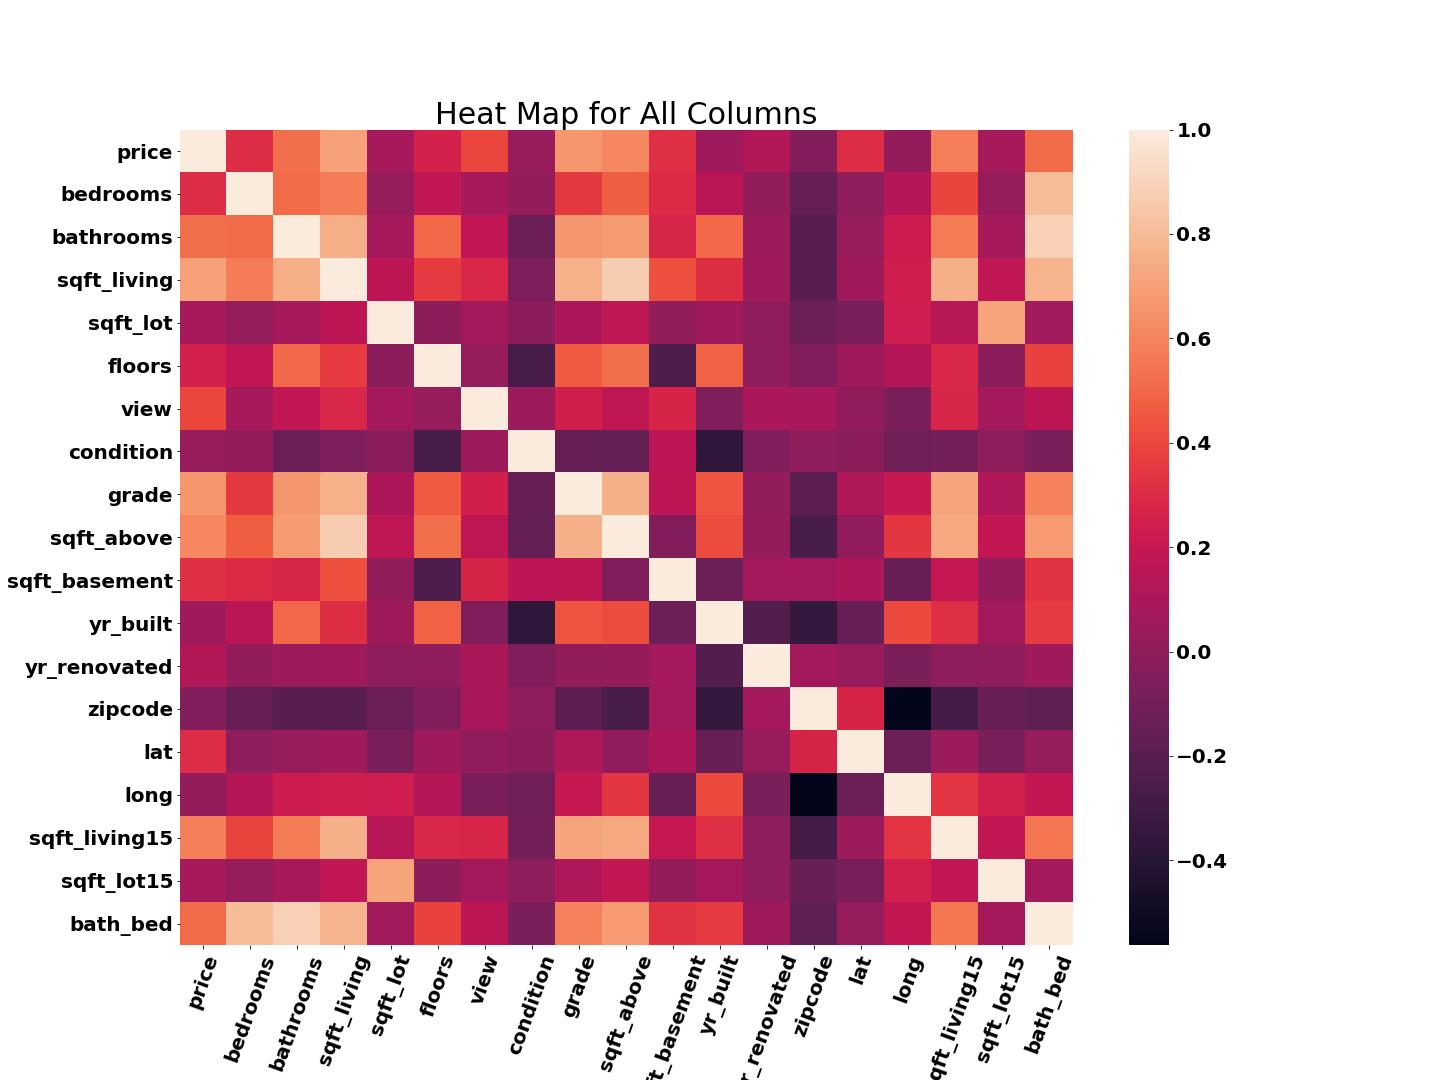
\includegraphics{heat_map.png}\label{heatmap}
			}
		\end{center}
	\end{itemize}
}
\section{Linear Model}
\subsection{Building the Linear Model}
\frame{
\frametitle{Selection of the explanatory variable for the Linear Model}
\begin{itemize}
	\item  ``sqft\_living'' has the highest correlation of  \(0.71\) with the ``price''. 
	\vskip 0.3in
	\pause
	\item  I build a regression model for the ``price'' to be predicted by ``sqft\_living''.
	\vskip 0.3in
	\pause 
	\item The model is \( \ln\left(\text{\it price}\right)  = 11.9524 + 0.0029 \cdot \text{\it sqft\_living}^{0.78}  \)
\end{itemize}
}
\subsection{Checking Statistical Hypotheses}
\frame{
\frametitle{Checking Statistical Hypotheses:}
This Linear Model satisfies all statistical assumptions of the Linear Regression, namely:
\begin{itemize}
	\item Linearity.
	\item Normality.
	\item There is no heteroscedasticity present in the model.
\end{itemize}
}
\subsection{Explanation of the Model}
\frame{
\frametitle{Intercept and slope }
Our model is 
\[ \ln\left(\text{\it price}\right)  = 11.9524 + 0.0029 \cdot \text{\it sqft\_living}^{0.78}  \]
\vspace{-0.2in}
\begin{itemize}
	\item The model has the sample intercept of \(11.9524\) and the slope of \(0.0029\).  
	\item To interpret the slope, we have to transform \(\hat{x}\) and \(\hat{y}\) towards original {\it sqft\_living} and {\it price}. 
\end{itemize}
\pause
To understand the change in {\it price} in percents we will use the following formula:
\begin{align*}
	Gab 100 \times \left[ e^{0.0029\left( x_2^{0.78} - x_1^{0.78} \right)} -1 \right]
\end{align*}
}
\frame{
	\frametitle{Example}
For example, if the {\it sqft\_living} is \(1000ft\) and we increase it to \(1100ft\), we will get the change in price of
\[100\times \left[e^{0.0029(1100^{0.78}-1000^{0.78})}-1\right] \approx 5.02\%. \]
\vskip 0.2in
\pause
In this particular example, \(10\%\) change in sqft\_living starting from \(x_1 = 1000ft\) forces \(5.02\%\) change in price.
}
\frame{
	\frametitle{\(R^2\)}
	\begin{itemize}
		\item The model has \(R^2\approx 0.45\).  
		\vskip 0.3in
		\pause
		\item This means that our model explains about 45\% of the variation by using {\it sqft\_living} as independent variable.
	\end{itemize}
}
\frame{
\frametitle{ANOVA}
Is our model with one explanatory variable better than the model with zero explanatory variables?\\
	\begin{itemize}
		\item Our p-value for this model is \(p=0.000 < 0.05 = \alpha\).
		 \vskip 0.1in
		 \item Since our p-value is \(0\), there is a \(0\%\) probability that the improvements that we are seeing with our one independent variable model are due to random chance alone.
	\end{itemize}
col}
\section{Multiple Linear Model}
\frame{
\frametitle{Multiple Linear Model}
Now, I will build a Multiple Regression Model.
\vskip 0.3in
The goals for Multiple Linear Model:
\vskip 0.2in
\begin{itemize}
	\item I want to improve $R^2$.
	\vskip 0.2in
	\item  I want to use more than one explanatory variable.
\end{itemize}
}
\frame{
\frametitle{Choice of Explanatory Variables}
I will use the highly correlated with the price features from the correlation matrix for the  Multiple Linear Model model.
\begin{center}
	\resizebox{0.6\textwidth}{!}{
		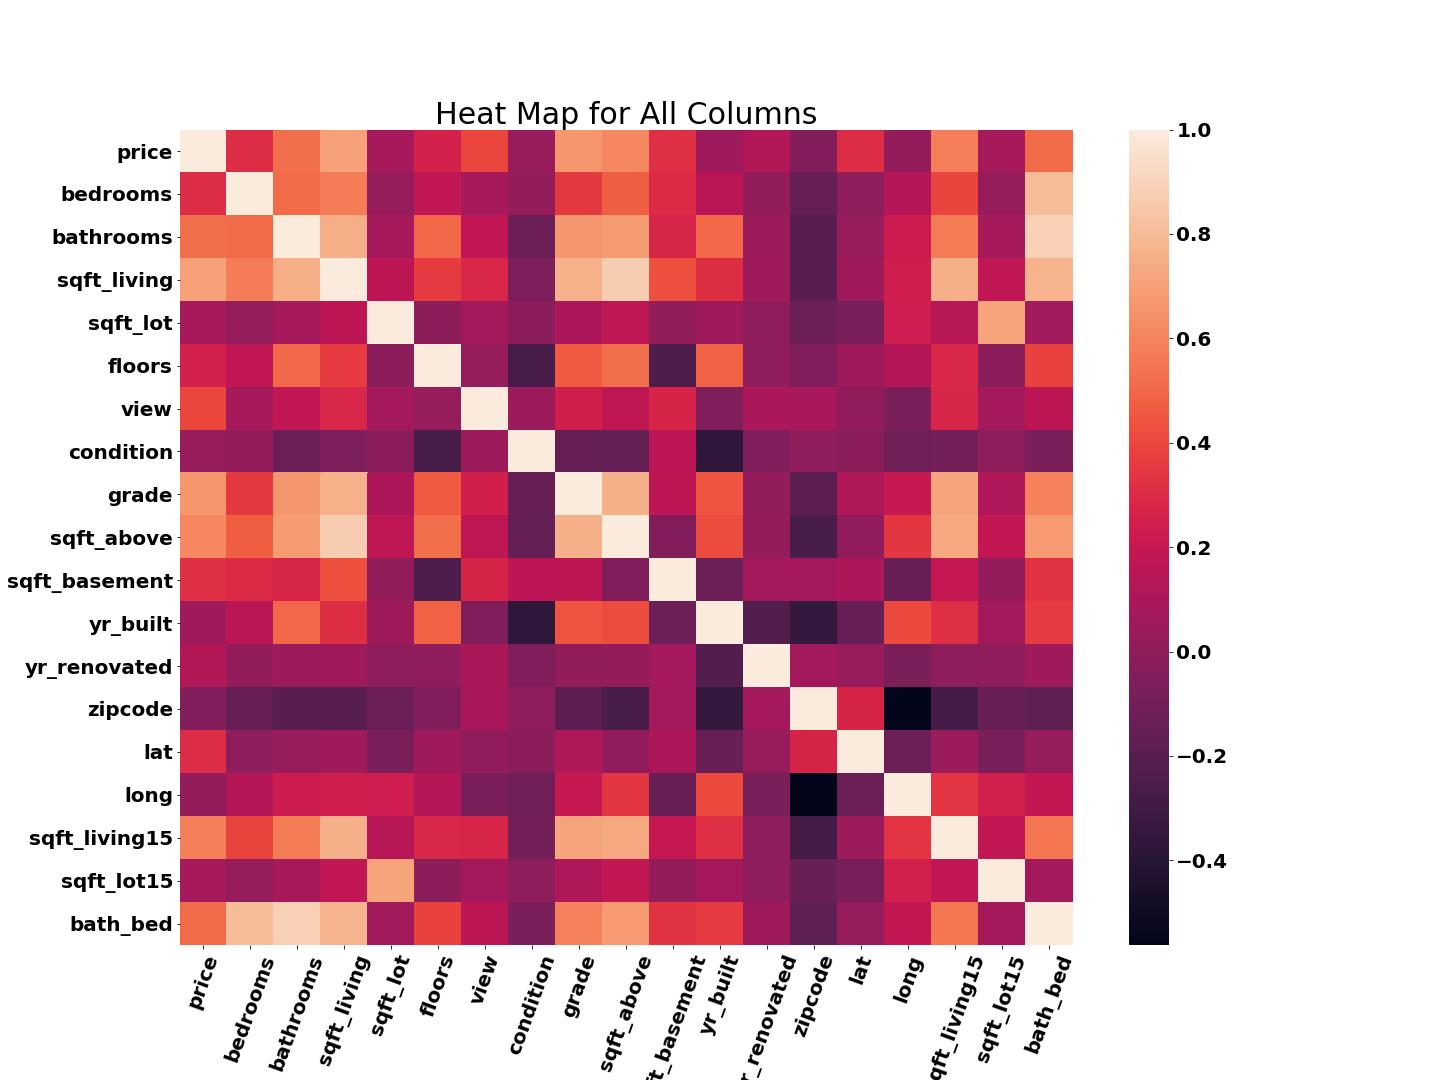
\includegraphics{heat_map.png}\label{heatmap}
	}
\end{center}
}
\subsection{Model}
\frame{
\frametitle{Results for Multiple Linear Regression Model}
At the end of my analysis, I came up with the following formula:
\pause
\vskip 0.2in
\begin{align*}
	\ln(price) =& 10.2082 + 0.3618\cdot \text{waterfront} - 0.0160\cdot\text{bedrooms}\\ -&0.0153 \cdot\text{bathrooms} +0.1400\cdot\text{sqft\_living}^{0.3}  + 0.0088 \cdot \text{floors}\\
	+& 0.1494\cdot\text{view}^{0.5}+ 0.0105\cdot\text{grade}^2+0.1187\cdot\ln\left(\text{sqft\_living15}\right)
\end{align*}
}
\subsection*{Check Statistical Hypotheses}
\frame{
	\frametitle{Check Statistical Hypotheses}
	This Linear Model satisfies all statistical assumptions of the Linear Regression, namely:
	\begin{itemize}
		\item Linearity.
		\item Normality.
	\end{itemize}
The model is very close to satisfy Constant Error Variance.
}

\frame{
	\frametitle{Overall Conclusion:}
	\begin{center}
		\textbf{ I conclude that our model almost satisfies statistical assumptions for the regression model.}
	\end{center}
}
\subsection{Explanation of the Model}
\frame{
\frametitle{Model}
\begin{align*}
	\ln(price) =& 10.2082 + 0.3618\cdot \text{waterfront} - 0.0160\cdot\text{bedrooms} \\-&
	0.0153 \cdot\text{bathrooms}  + 0.1400\cdot\text{sqft\_living}^{0.3} + 0.0088 \cdot \text{floors}\\
	+& 0.1494\cdot\text{view}^{0.5}+ 0.0105\cdot\text{grade}^2+0.1187\cdot\ln\left(\text{sqft\_living15}\right)
\end{align*}
}
\frame{
\frametitle{Explanation of the Model}
Before I begin explain the coefficients, I notice that $P>|t|$ for the {\it floors} variable is $0.155$, which makes  {\it floors} insignificant for the analysis. 
}
\frame{
\frametitle{Intercept}
\begin{itemize}
	\item  The model has the sample intercept of $10.2082$.
	\vskip 0.3in 
	\pause
	\item If we assume that all explanatory variables are zeros, this would mean that the price would be $e^{10.2082}\approx 27,124$
\end{itemize}
}
\frame{
\frametitle{$0.3618$ is the coefficient for {\it waterfront}}
{\it Waterfront} is a categorical variable coded as $0$ or $1$.
\vskip 0.1in
\pause 
To understand the change in {\it price} in percents, if we switch from the house with no waterfront to the house with waterfront while keeping all other variables the same, will use the following formula:
$$
100\times \left[ e^{0.3618} - 1\right] \approx 43.59\%
$$
\vskip 0.1in
\pause
Switching from the house with no waterfront to the house with waterfront while keeping all other explanatory variables fixed, will increase the price by 43.59\%.

}
\frame{
\frametitle{$0.1400$ is the coefficient for {\it sqft\_living}}
If we increase the {\it sqft\_living} from $1000ft$ to $1100ft$ while keeping the other variables fixed, we will get the following change in price in percents:
$$
100 \times \left[ e^{0.1400 \left( 1100^{0.3} - 1000^{0.3}\right)} - 1 \right]\approx 3.28\%
$$
\begin{itemize}
	\item If the {\it sqft\_living} is $1000ft$ and we increase it to $1100ft$ while keeping the other variables fixed, we will get the change in price of $3.28\%$.
	\vskip 0.3in
	\pause
	\item In this particular example $10\%$ change in {\it sqft\_living} starting from $1000ft$ forces $3.28\%$ change in price.
\end{itemize}
}
\frame{
	\frametitle{$0.1494$ is the coefficient for the {\it view}}
	The coefficient for the {\it view} has the same explanation as the {\it sqft\_living}. 
	\vskip 0.3in
	\pause
	If we increase the {\it view} by $1$ unit from $2$ to $3$ while keeping the other variables fixed, we will get the following:
	$$
 	100 \times \left[ e^{0.1494 \left( 3^{0.5} - 2^{0.5}\right)} - 1 \right]\approx 4.86\%
	$$
	In this particular example if the {\it view} will increase from $2$ to $3$, the price will increase by 4.86\%.
}
\frame{
\frametitle{$0.0105$ is the coefficient for the {\it grade}}
 The coefficient for the {\it grade} has the same explanation as the {\it sqft\_living}.
 \vskip 0.3in
 \pause
  If we increase the {\it grade} by $1$ unit from $2$ to $3$ while keeping the other variables fixed, we will get the following:
$$
 100 \times \left[ e^{0.0105\left( 3^{2} - 2^{2}\right)} - 1 \right]\approx 5.39\%
$$
In this particular example if the {\it grade} will increase from $2$ to $3$ while other variables stay the same, the price will increase by 5.39\%.
}
\frame{
\frametitle{$0.1187$ is the coefficient for the {\it sqft\_living15}}
The change in price in percent will be:
$$
 100 \times \left[ \left(\frac{\text{price 2}}{\text{price 1}}\right)^{0.1187} - 1 \right]
$$
In this particular example, if we increase the {\it sqft\_living15} by $100$ units from $1000$ to $1100$ while keeping the other variables fixed, we will get the following:
$$
100 \times \left[ e^{0.1187}\times \frac{1100}{1000} - 1 \right] \approx 1.14\%
$$
Thus, 10\% increase in {\it sqft\_living15} will lead to 1.14\% increase in {\it price}.
}
\frame{
	\frametitle{\(R^2\)}
	\begin{itemize}
		\item The model has \(R^2\approx 0.5\).  
		\vskip 0.3in
		\pause
		\item This means that our model explains about 50\% of the variation by using {\it sqft\_living} as independent variable.
	\end{itemize}
}
\frame{
\frametitle{ANOVA}
Is our model with many explanatory variable better than the model with zero explanatory variables?\\
\begin{itemize}
	\item Our p-value for this model is \(p=0.000 < 0.05 = \alpha\). 
	\item We conclude that the Test tells us, that at least one of the coefficients is not $0$. 
	\item Since our p-value is $0$, there is a $0\%$ probability that the improvements that we are seeing with our independent variables model are due to random chance alone.
\end{itemize}
}
\section{Conclusions}
\subsection{Data Modeling}
\begin{frame}
	\frametitle{Conclusions: Data Modeling}
	 I used the following steps during data modeling:
	\begin{itemize}
		\item  Dropped 2376 rows where {\it waterfront} has no value.
		\item  Dropped 63 rows where {\it view} is has no value.
		\item Dropped 3842 rows where {\it yr\_renovated} has no value.
		\item I converted {\it sqft\_basement}  string format into numeric values.
		\item  During modeling I dropped very large and very small values when necessary.
	\end{itemize}
\end{frame}
\subsection{Modeling}
\frame{
\frametitle{Conclusions: Modeling}
\begin{itemize}
	\item I built two models:
	\begin{itemize}
		\item  Linear Regression Model
		\item Multiple Linear Regression Model
	\end{itemize}
	\item  I checked whether the models satisfy statistical assumptions of Linear Regression
	\item  I explained the models.
	\item Models can be used for interpolation given the data about a particular property.
\end{itemize}
}
\subsection{Ways to improve the analysis}
\frame{
\frametitle{Conclusions: Ways to Improve the Analysis}
\begin{itemize}
	\item More data wrangling is need to remove {\it heteroscedasticity} from the Multiple Linear Regression Model.
	\item  Include more explanatory variables.
	\item Scrape webpages for more data such as school grade, crime rate, etc. for properties.
\end{itemize}
}
\frame{
\begin{center}
	\LARGE
	THE END \\
	THANK YOU!
\end{center}
}
\end{document}